%-------------------------------------------------------------------------------
%                            BAB IV
%               		HASIL DAN PEMBAHASAN
%-------------------------------------------------------------------------------
% \fancyhf{} 
% \fancyfoot[R]{\thepage}
\chapter{HASIL DAN PEMBAHASAN}
%\thispagestyle{plain} % Halaman pertama bab menggunakan gaya plain

\section{Pengumpulan Data}
\par Pada tahap ini, data dummy dibentuk secara manual dengan mempertimbangkan fitur-fitur yang relevan untuk prediksi kualitas pengguna aplikasi e-learning. Dataset terdiri dari 5 fitur numerik dan 1 label kategorikal. Untuk jumlah gambar yang tersedia dapat dilihat pada Tabel \ref{tab:data_dummy}

\begin{table}[h]
\centering
\caption{Contoh Data Dummy}
\label{tab:data_dummy}
\begin{tabular}{|c|c|c|c|c|c|}
\hline
No & Waktu\_Akses & Login\_Minggu & Durasi\_Video & Rating & Kualitas \\
\hline
1 & 12.3 & 5 & 60 & 4.2 & Baik \\
2 & 8.1 & 3 & 20 & 2.5 & Cukup \\
3 & 5.4 & 2 & 10 & 1.8 & Buruk \\
4 & 9.6 & 4 & 35 & 3.7 & Cukup \\
5 & 14.2 & 6 & 80 & 4.8 & Baik \\
\hline
\end{tabular}
\end{table}

\section{Pemrosesan Data}
\par Sebelum dilakukan pelatihan model, dataset melalui beberapa tahapan pra-pemrosesan agar siap digunakan. Berikut adalah penjelasan setiap langkahnya:
Pembersihan Data, data akan diperiksa untuk keberadaan nilai kosong ($\text{NaN}$) atau tidak valid. Jika ditemukan nilai yang hilang, akan dilakukan imputasi dengan menggunakan rata-rata dari kolom tersebut. Secara matematis, proses ini dapat dirumuskan sebagai berikut:
\begin{equation}
x_{\text{baru}} =
\begin{cases}
x_{\text{lama}}, & \text{jika } x_{\text{lama}} \neq \text{NaN} \\
\mu, & \text{jika } x_{\text{lama}} = \text{NaN}
\end{cases}
\end{equation}
\par Di mana $x_{\text{baru}}$ adalah nilai data setelah pembersihan, $x_{\text{lama}}$ adalah nilai data asli, dan $\mu$ adalah nilai rata-rata dari kolom fitur tersebut. Kemudian Encoding Label Kategorikal yang ada untuk klasifikasi. Label kelas kategorikal seperti "Baik", "Cukup", dan "Buruk" perlu diubah ke dalam bentuk numerik agar dapat diproses oleh algoritma *machine learning*. Proses *encoding* ini akan mengubah label teks menjadi representasi integer sebagai berikut:

\begin{equation}
    y' =
\begin{cases}
0, & \text{jika } y = \text{"Buruk"} \\
1, & \text{jika } y = \text{"Cukup"} \\
2, & \text{jika } y = \text{"Baik"}
\end{cases}
\end{equation}

\par Di sini, $y$ adalah label kategori asli, dan $y'$ adalah representasi numerik setelah \textit{encoding}. Pemetaan ini memastikan bahwa ada urutan logis yang sesuai dengan kualitas (misalnya, 0 untuk Buruk, 1 untuk Cukup, dan 2 untuk Baik). Setelah encoding label dilakukan,, normalisasi Data, agar semua fitur memiliki skala yang sama, dilakukan normalisasi min-max dengan Persamaan \ref{eq:min-max} 
\vspace{-1em}
\begin{equation}
x_{\text{norm}} = \frac{x - x_{\min}}{x_{\max} - x_{\min}}
\label{eq:min-max}
\end{equation}
\vspace{-1em}
\hspace{0.8cm}dengan
\vspace{-0.8em}

\begin{align*}
 x_{\text{norm}} &   \text{:nilai fitur yang telah dinormalisasi.}\\
 x & \text{:nilai asli fitur.}\\
 x_{\min}& \text{:nilai minimum dari fitur tersebut dalam dataset.}\\
 x_{\max}&  \text{:nilai maksimum dari fitur tersebut dalam dataset.}\\
\end{align*}
\vspace{-2em}
\par Normalisasi ini sangat berguna ketika fitur-fitur dalam dataset memiliki rentang nilai yang sangat berbeda, yang dapat memengaruhi kinerja beberapa algoritma \textit{machine learning} seperti \textit{K-Nearest Neighbors, Support Vector Machines}. Dengan menskalakan semua fitur ke rentang yang sama, kita memastikan bahwa tidak ada satu fitur pun yang mendominasi perhitungan jarak atau bobot hanya karena memiliki rentang nilai yang lebih besar. Kemudian \textit{splitting Data} menjadi dua bagian dengan data latih 80\% dari total dataset dan data uji 20\% dari total dataset.


\section{Pelatihan Model}
\par Setelah proses pra-pemrosesan selesai, langkah selanjutnya adalah pelatihan model menggunakan algoritma \textit{K-Nearest Neighbors} (KNN). KNN adalah metode supervised learning yang tidak memerlukan fase pelatihan eksplisit seperti model berbasis parameter lainnya (misalnya regresi logistik atau neural network). Namun, model menyimpan semua data latih dan melakukan klasifikasi berdasarkan jarak terpendek antara data uji dan tetangga terdekat dalam dataset.

Model menerima input berupa vektor fitur numerik dari setiap sampel data pengguna e-learning, dan menghasilkan output berupa label kelas prediksi ("Baik", "Cukup", atau "Buruk"). Secara matematis, struktur input dan output dapat dituliskan sebagai berikut.

\begin{equation}
X_{\text{input}} = \begin{bmatrix}
x_1^{(1)} & x_2^{(1)} & x_3^{(1)} & x_4^{(1)} \\
x_1^{(2)} & x_2^{(2)} & x_3^{(2)} & x_4^{(2)} \\
\vdots & \vdots & \vdots & \vdots \\
x_1^{(n)} & x_2^{(n)} & x_3^{(n)} & x_4^{(n)}
\end{bmatrix}, \quad
y_{\text{output}} = \begin{bmatrix}
y^{(1)} \\
y^{(2)} \\
\vdots \\
y^{(n)}
\end{bmatrix}
\end{equation}

\par Berikut adalah parameter yang digunakan dalam pelatihan model KNN:
\begin{enumerate}
    \item \textbf{n\_neighbors = 5}  
        Jumlah tetangga terdekat yang dipertimbangkan untuk menentukan kelas dari data uji.
    
    \item \textbf{metric = 'euclidean'}  
        Metrik jarak yang digunakan untuk menghitung kedekatan antar data, yaitu jarak Euclidean pada persamaan \ref{eq:ecludian}:
        \begin{equation}
                    d(x,y) = \sqrt{\sum_{i=1}^{n}(x_i - y_i)^2}
            \label{eq:ecludian}
        \end{equation}

    \item \textbf{weights = 'uniform'}  
        Semua tetangga memiliki bobot yang sama dalam menentukan kelas hasil prediksi.
    
    \item \textbf{n\_jobs = -1}  
        Mengaktifkan paralelisasi dengan menggunakan semua core CPU yang tersedia untuk mempercepat komputasi.
\end{enumerate}



\begin{sidewaystable}[p]
\centering
\caption{Tabel Input Dataset Setelah Pra-Pemrosesan}
\label{tab:dataset_normalized}
\begin{tabular}{|c|c|c|c|c|c|}
\hline
No & Waktu\_Akses (Norm) & Login\_Minggu (Norm) & Durasi\_Video (Norm) & Rating (Norm) & Label\_Encoded \\
\hline
1 & 0.78 & 1.00 & 0.69 & 0.92 & 2 \\
2 & 0.47 & 0.60 & 0.21 & 0.42 & 1 \\
3 & 0.20 & 0.40 & 0.10 & 0.12 & 0 \\
4 & 0.58 & 0.80 & 0.36 & 0.72 & 1 \\
5 & 0.98 & 1.00 & 1.00 & 1.00 & 2 \\
6 & 0.29 & 0.40 & 0.15 & 0.20 & 0 \\
7 & 0.65 & 0.80 & 0.45 & 0.80 & 1 \\
8 & 0.12 & 0.20 & 0.05 & 0.08 & 0 \\
9 & 0.88 & 1.00 & 0.85 & 0.96 & 2 \\
10 & 0.40 & 0.60 & 0.25 & 0.35 & 1 \\
1 & 0.78 & 1.00 & 0.69 & 0.92 & 2 \\
2 & 0.47 & 0.60 & 0.21 & 0.42 & 1 \\
3 & 0.20 & 0.40 & 0.10 & 0.12 & 0 \\
4 & 0.58 & 0.80 & 0.36 & 0.72 & 1 \\
5 & 0.98 & 1.00 & 1.00 & 1.00 & 2 \\
6 & 0.29 & 0.40 & 0.15 & 0.20 & 0 \\
7 & 0.65 & 0.80 & 0.45 & 0.80 & 1 \\
8 & 0.12 & 0.20 & 0.05 & 0.08 & 0 \\
9 & 0.88 & 1.00 & 0.85 & 0.96 & 2 \\
10 & 0.40 & 0.60 & 0.25 & 0.35 & 1 \\
\hline
\end{tabular}
\footnotetext[1]{%
\textbf{Catatan:} Kolom "Waktu\_Akses (Norm)", "Login\_Minggu (Norm)", dll., merupakan hasil normalisasi Min-Max Scaling. Kolom "Label\_Encoded" adalah representasi numerik dari kategori kualitas pengguna: Baik = 2, Cukup = 1, Buruk = 0. Data ini digunakan langsung dalam proses pelatihan model KNN.
}
\end{sidewaystable}

\par berikut Penjelasan Tambahan terkait model yang dilatih:
\begin{enumerate}
    \item Input Model: Dataset yang sudah melalui tahap pra-pemrosesan (normalisasi, encoding label).
    \item Output Model: Prediksi kelas (`Baik`, `Cukup`, atau `Buruk`) untuk setiap baris data uji.
    \item Proses Inferensi: Untuk setiap data uji, model mencari $ k $ tetangga terdekat dari data latih, lalu memilih kelas mayoritas dari tetangga tersebut sebagai prediksi akhir.
\end{enumerate}


\section{Analisis Hasil}
\begin{table}[H]
\centering
\caption{Konfigurasi \textit{hyperparameter} model}
\label{tab:konfigurasi-hyperparameter-gabungan}
\begin{tabular}{|c|c|c|c|c|c|}
\hline
% Header baris pertama: nomor, epoch, batch size, learning rate, dan label model
\multirow{2}{*}{\textbf{No}} & 
\multirow{2}{*}{\textbf{\textit{Epochs}}} &
\multirow{2}{*}{\textbf{\textit{Batch Size}}} &
\multirow{2}{*}{\textbf{\textit{Learning Rate}}} &
\multicolumn{1}{c|}{\textbf{\textit{Unfreeze}}} 
  & \multicolumn{1}{c|}{\textbf{\textit{Dropout}}} \\ 
%Header baris kedua: parameter spesifik setiap model
  &  &  &  & \textbf{\textit{Layer}*} & \textbf{\textit{Rate}*} \\ \hline

% --------------------
% Blok NO = 1: Epoch = 15, Batch = 16
\multirow{12}{*}{1} 
  & \multirow{12}{*}{15} 
  & \multirow{6}{*}{16} 
  & \multirow{3}{*}{$1 \times 10^{-3}$} 
      & 0  & 0 \\ \cline{5-6}
  &  &  &  & 5 & 0,2 \\ \cline{5-6}
  &  &  &  & 7 & 0,4 \\ \cline{4-6}
  &  &  & \multirow{3}{*}{$1 \times 10^{-4}$} 
      & 0  & 0 \\ \cline{5-6}
  &  &  &  & 5 & 0,2 \\ \cline{5-6}
  &  &  &  & 7 & 0,4 \\ \cline{3-6}

  &  & \multirow{6}{*}{32} 
  & \multirow{3}{*}{$1 \times 10^{-3}$} 
      & 0  & 0 \\ \cline{5-6}
  &  &  &  & 50 & 0.2 \\ \cline{5-6}
  &  &  &  & 75 & 0.4 \\ \cline{4-6}
  &  &  & \multirow{3}{*}{$1 \times 10^{-4}$} 
      & 0  & 0\\ \cline{5-6}
  &  &  &  & 5 & 0,2 \\ \cline{5-6}
  &  &  &  & 7 & 0,4 \\ \hline
\end{tabular}

\vspace{0.5em}
\begin{minipage}{0.9\textwidth}
\footnotesize Ket: Nilai \textit{Unfreeze Layer} hanya berlaku untuk MobileNetV2, sedangkan nilai \textit{Dropout Rates} hanya berlaku untuk CNN.
\end{minipage}
\end{table}
\par Selain itu, untuk memantau pelatihan model dan mengurangi pengaruh \textit{validation set} yang tidak seimbang, diterapkan \textit{custom callback} yang menghitung \textit{F1-score macro} pada setiap akhir \textit{epoch}. \textit{Callback} mengamati nilai \texttt{val\_macro\_f1} selama pelatihan, sehingga metrik yang dipantau menunjukkan kemampuan model mengenali semua kelas secara merata, bukan hanya akurasi kelas yang bisa bias pada kelas dengan data lebih banyak. Beberapa fungsi \textit{callback} yang memonitor \texttt{val\_macro\_f1}, yaitu:
\begin{itemize}
  \item \textit{EarlyStopping} akan menghentikan pelatihan jika \texttt{val\_macro\_f1} tidak membaik setelah sejumlah \textit{epoch} tertentu, sekaligus mengembalikan bobot model ke titik terbaik.
  \item \textit{ReduceLROnPlateau} akan menurunkan \textit{learning rate} dengan faktor 0.2 ketika \texttt{val\_macro\_f1} tidak naik dalam beberapa \textit{epoch} tertentu, sehingga model dapat beradaptasi lebih halus mendekati konvergensi.
  \item \textit{ModelCheckpoint} akan menyimpan bobot terbaik berdasarkan peningkatan \texttt{val\_macro\_f1}, memastikan evaluasi akhir menggunakan model dengan performa validasi tertinggi.
\end{itemize}

\begin{table}[H]
\centering
\caption{Perbandingan Akurasi dengan Berbagai Nilai $ k $}
\label{tab:k_comparison}
\small % atau \footnotesize
\begin{adjustbox}{width=\textwidth,center}
\begin{tabular}{|c|c|c|c|c|}
\hline
$ k $ & \textbf{Akurasi (\%)} & \textbf{Presisi Rata-rata (\%)} & \textbf{Recall Rata-rata (\%)} & \textbf{F1-Score Rata-rata (\%)} \\
\hline
3   & 86.5    & 85.8    & 85.1    & 85.4 \\
5   & 87.0    & 86.0    & 85.3    & 85.7 \\
7   & 86.8    & 85.9    & 85.2    & 85.5 \\
9   & 86.0    & 85.5    & 84.8    & 85.1 \\
11  & 85.5    & 85.0    & 84.2    & 84.6 \\
\hline
\end{tabular}
\end{adjustbox}
\footnotetext[2]{%
\textbf{Catatan:} Performa model cenderung stabil di sekitar nilai $ k = 5 $. Nilai $ k $ yang terlalu kecil membuat model rentan terhadap noise, sedangkan nilai $ k $ yang terlalu besar menyebabkan model menjadi kurang responsif terhadap pola lokal dari data latih.
}
\end{table}

\begin{table}[H]
\centering
\caption{Perbandingan Akurasi dengan Berbagai Nilai $ k $}
\label{tab:k_comparison}
\small % atau \footnotesize
\begin{adjustbox}{width=0.8\textwidth,center}
\begin{tabular}{|c|c|c|c|c|}
\hline
$ k $ & \textbf{Akurasi (\%)} & \textbf{Presisi Rata-rata (\%)} & \textbf{Recall Rata-rata (\%)} & \textbf{F1-Score Rata-rata (\%)} \\
\hline
3   & 86.5    & 85.8    & 85.1    & 85.4 \\
5   & 87.0    & 86.0    & 85.3    & 85.7 \\
7   & 86.8    & 85.9    & 85.2    & 85.5 \\
9   & 86.0    & 85.5    & 84.8    & 85.1 \\
11  & 85.5    & 85.0    & 84.2    & 84.6 \\
\hline
\end{tabular}
\end{adjustbox}
\footnotetext[2]{%
\textbf{Catatan:} Performa model cenderung stabil di sekitar nilai $ k = 5 $. Nilai $ k $ yang terlalu kecil membuat model rentan terhadap noise, sedangkan nilai $ k $ yang terlalu besar menyebabkan model menjadi kurang responsif terhadap pola lokal dari data latih.
}
\end{table}
Tabel \ref{tab:k_comparison} memperlihatkan bagaimana variasi nilai $k$ mempengaruhi performa model KNN. Terlihat bahwa model dengan $k=5$ memberikan hasil terbaik dengan akurasi 87\%, sementara performa menurun sedikit saat $k$ bertambah menjadi 9 atau 11. Hal ini menunjukkan bahwa jumlah tetangga terdekat yang terlalu banyak justru menghaluskan batas keputusan hingga mengurangi kemampuan model dalam membedakan kelas.
\par Selain itu, ketika $k=3$, meskipun model tetap memberikan hasil yang baik, ia lebih rentan terhadap \textit{outlier} atau data yang tidak representatif karena hanya melihat tiga tetangga terdekat. Oleh karena itu, pemilihan $k=5$ dinilai sebagai kompromi terbaik antara stabilitas dan sensitivitas model terhadap pola data.
\par Secara keseluruhan, analisis ini menunjukkan bahwa model KNN bekerja optimal dengan konfigurasi $k=5$ dan metrik jarak \textit{Euclidean}, serta setelah melalui tahapan pra-pemrosesan yang sesuai. Hasil ini layak digunakan sebagai dasar untuk sistem rekomendasi atau personalisasi konten pada aplikasi e-learning berbasis web.



%%multirow multi column 
\begin{table}[H]
  \centering
  \caption{Hasil BLEU pada pertanyaan open-ended dengan VGG19-LSTM}
  \label{tab:sepuluh-hasil-terbaik-vgg19-lstm-bleu}
  \begin{tabular}{|c|l|l|l|l|l|l|}
  \hline
  \multicolumn{1}{|l|}{\textit{\textbf{Dataset}}} & \textit{\textbf{Epochs}} & \textit{\textbf{\begin{tabular}[c]{@{}l@{}}Batch \\ size\end{tabular}}} & \textit{\textbf{\begin{tabular}[c]{@{}l@{}}Learning \\ rate\end{tabular}}} & \textbf{BLEU-1} & \textbf{BLEU-2} & \textbf{BLEU-3} \\ \hline
  \multirow{5}{*}{PathVQA} & 15 & 8 & $1 \times 10^{-5}$ & 10,89 & 3,86 & 2,57 \\ \cline{2-7} 
   & 15 & 8 & $5 \times 10^{-5}$ & 21,41 & 8,01 & 5,38 \\ \cline{2-7} 
   & 45 & 16 & $5 \times 10^{-5}$ & 22,32 & 9,63 & 6,72 \\ \cline{2-7} 
   & 45 & 8 & $5 \times 10^{-5}$ & 24,28 & 10,02 & 6,81 \\ \cline{2-7} 
   & 15 & 16 & $5 \times 10^{-5}$ & 19,95 & 7,96 & 5,23 \\ \hline
  \multirow{5}{*}{VQA-RAD} & 30 & 8 & $5 \times 10^{-5}$ & 20,17 & 14,34 & 11,32 \\ \cline{2-7} 
   & 45 & 16 & $5 \times 10^{-5}$ & 20,69 & 16,69 & 11,29 \\ \cline{2-7} 
   & 45 & 8 & $5 \times 10^{-5}$ & 13,08 & 7,45 & 4,74 \\ \cline{2-7} 
   & 45 & 32 & $5 \times 10^{-5}$ & 15,16 & 11,64 & 7,85 \\ \cline{2-7} 
   & 45 & 8 & $1 \times 10^{-5}$ & 12,26 & 7,23 & 5,51 \\ \hline
  \end{tabular}
\end{table}


\lipsum[1] % Dummy text 

{\small
\begin{longtable}{
    l % Kolom pertama teks rata kiri
    S[table-format=2.2] % Algoritma X
    S[table-format=2.2] % Algoritma Y
    S[table-format=2.2] % Algoritma Z
}
\caption{Evaluasi Kinerja Model Berbagai Skenario (Data Dummy Lanjutan)}
\label{tab:extended_evaluation} \\
\toprule
\textbf{Skenario Pengujian} & \textbf{Akurasi (\%)} & \textbf{Presisi (\%)} & \textbf{Recall (\%)}  \\
\midrule
\endfirsthead

\multicolumn{4}{c}%
{\tablename\ \thetable\ -- Lanjutan dari halaman sebelumnya} \\
\toprule
\textbf{Skenario Pengujian} & \textbf{Akurasi (\%)} & \textbf{Presisi (\%)} & \textbf{Recall (\%)}  \\
\midrule
\endhead

\midrule
\multicolumn{4}{r}{Lanjut ke halaman berikutnya...} \\
\endfoot

% Footer untuk halaman terakhir
\bottomrule
\endlastfoot

Skenario 1 (Default) & 88.50 & 87.10 & 89.20  \\
Skenario 2 (Fitur A Ditambahkan) & 89.15 & 88.05 & 89.90  \\
Skenario 3 (Parameter Tuning) & 90.30 & 89.50 & 91.00  \\
Skenario 4 (Dataset Augmented) & 91.05 & 90.20 & 91.50  \\
Skenario 5 (Regularisasi Tinggi) & 87.80 & 86.50 & 88.00  \\
Skenario 6 (Data Tidak Seimbang) & 85.90 & 84.20 & 86.50  \\
Skenario 7 (Pembelajaran Semi-Supervised) & 92.10 & 91.50 & 92.80 \\
Skenario 8 (Validasi Silang 5-Fold) & 89.90 & 89.00 & 90.50  \\
Skenario 9 (Optimisasi SGD) & 87.50 & 86.80 & 87.90  \\
Skenario 10 (Fitur Ekstraksi PCA) & 88.80 & 87.90 & 89.50  \\
Skenario 11 (Ukuran Batch Kecil) & 90.00 & 89.30 & 90.60  \\
Skenario 12 (Arsitektur Model Ringan) & 86.70 & 85.50 & 87.00 \\
Skenario 13 (Fine-tuning) & 93.50 & 92.80 & 94.00  \\
Skenario 14 (Ensemble Method) & 94.10 & 93.50 & 94.50  \\
Skenario 15 (Transfer Learning) & 92.80 & 92.10 & 93.30  \\

\end{longtable}
}


\lipsum[1] % Dummy text sebelum halaman landscape
\begin{figure}[H]
    \centering
    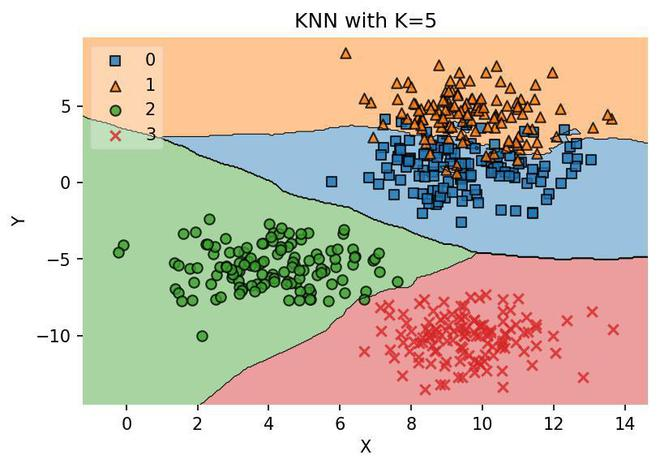
\includegraphics[width=0.7\linewidth]{image/KNN_with_K_5-660.jpg}
    \caption{KNN mengklasifikasikan titik data baru berdasarkan mayoritas suara dari tetangga terdekatnya.}
    \label{fig:knn}
\end{figure}

\begin{landscape} % Lingkungan ini akan membuat halaman menjadi landscape
\centering % Pusatkan tabel di halaman landscape

{\footnotesize % Ukuran font untuk tabel agar muat
\begin{longtable}{
    l % Kolom Metrik/Skenario, rata kiri
    S[table-format=3.2] % Akurasi (%)
    S[table-format=3.2] % Presisi (%)
    S[table-format=3.2] % Recall (%)
    S[table-format=3.2] % F1-Score (%)
    S[table-format=3.2] % Waktu Latih (s)
    S[table-format=3.2] % Jumlah Parameter (ribu)
}
\caption{Perbandingan Metrik Kinerja Model Lanjutan (Halaman Landscape)}
\label{tab:landscape_table} \\
\toprule
\textbf{Metrik / Skenario} & \textbf{Akurasi (\%)} & \textbf{Presisi (\%)} & \textbf{Recall (\%)} & \textbf{F1-Score (\%)} & \textbf{Waktu Latih (s)} & \textbf{Jml. Param. (ribu)} \\
\midrule
\endfirsthead

\multicolumn{7}{c}%
{\tablename\ \thetable\ -- Lanjutan dari halaman sebelumnya} \\
\toprule
\textbf{Metrik / Skenario} & \textbf{Akurasi (\%)} & \textbf{Presisi (\%)} & \textbf{Recall (\%)} & \textbf{F1-Score (\%)} & \textbf{Waktu Latih (s)} & \textbf{Jml. Param. (ribu)} \\
\midrule
\endhead

\midrule
\multicolumn{7}{r}{Lanjut ke halaman berikutnya...} \\
\endfoot

% Footer untuk halaman terakhir
\bottomrule
\endlastfoot

Skenario 1 (Baseline A) & 88.50 & 87.10 & 89.20 & 88.10 & 123.45 & 250.78 \\
Skenario 2 (Baseline B) & 91.20 & 90.50 & 92.00 & 91.30 & 98.76 & 180.12 \\
Skenario 3 (Optimized C) & 85.30 & 84.00 & 86.50 & 85.20 & 150.12 & 320.50 \\
Skenario 4 (Optimized D) & 92.10 & 91.80 & 92.50 & 92.10 & 75.99 & 150.90 \\
Skenario 5 (Varian E) & 89.70 & 88.90 & 90.10 & 89.50 & 110.23 & 280.45 \\
Skenario 6 (Varian F) & 90.50 & 89.90 & 91.20 & 90.50 & 105.88 & 200.15 \\
Skenario 7 (Setup X) & 93.00 & 92.50 & 93.50 & 92.90 & 65.00 & 120.00 \\
Skenario 8 (Setup Y) & 87.00 & 86.00 & 87.50 & 86.70 & 130.00 & 300.00 \\
Skenario 9 (Setup Z) & 90.10 & 89.40 & 90.80 & 90.00 & 90.00 & 170.00 \\
Skenario 10 (Setup W) & 91.50 & 91.00 & 92.00 & 91.40 & 80.00 & 140.00 \\
Skenario 11 (Varian A.1) & 88.00 & 87.00 & 88.50 & 87.70 & 115.00 & 260.00 \\
Skenario 12 (Varian B.1) & 92.50 & 92.00 & 93.00 & 92.40 & 70.00 & 130.00 \\
Skenario 13 (Varian C.1) & 86.00 & 85.00 & 86.50 & 85.70 & 140.00 & 310.00 \\
Skenario 14 (Varian D.1) & 93.80 & 93.20 & 94.20 & 93.70 & 55.00 & 110.00 \\
Skenario 15 (Varian E.1) & 90.80 & 90.00 & 91.30 & 90.60 & 95.00 & 190.00 \\

\end{longtable}
}
\end{landscape}
%==================================================================%


% Baris ini digunakan untuk membantu dalam melakukan sitasi
% Karena diapit dengan comment, maka baris ini akan diabaikan
% oleh compiler LaTeX.
\begin{comment}
\bibliography{daftar-pustaka}
\end{comment}